%%%%%%%%%%%%%%%%%%%%%%%%%%%%%%%%%%%%%%%%%%%%%%%%%%%%%%%%%%%%%%%%%%%%%%%%%%%%%
%	e-Yantra, IIT-Bombay

%	Document Author: Abhishek Rathore, Gopineedi Harsha Vardhan
%	Date: 07-June,2016 

%%%%%%%%%%%%%%%%%%%%%%%%%%%%%%%%%%%%%%%%%%%%%%%%%%%%%%%%%%%%%%%%%%%%%%%%%%%%%

\documentclass[11pt,a4paper]{article}

\usepackage{graphicx}
\usepackage{listings}
\usepackage{url}
\title{Tutorial - Colored object tracking using HSV}
\author{e-Yantra Team}
\date{\today}

\begin{document}
	\maketitle
	\newpage
	\tableofcontents
	\newpage
	\section{Colored object tracking using HSV}
	The objective of this tutorial is to track a colored object. We track the object whose color lies in the specified range of HSV color space values using largest contour inside the frame.
	\section{Prerequisites}
	User should have handy knowledge of following before reading this tutorial.
	\begin{itemize}
		\item Basics of Python Language.
		\item Introduction to OpenCV.
		\item Basics of Image processing in OpenCV using Python.
		\item Knowledge on BGR and HSV color space and interconversion.
	\end{itemize}
	\section{Hardware Requirement}
	\begin{itemize}
		\item A Computer with internal or external webcam.
	\end{itemize}
	\section{Software Requirement}
	\begin{itemize}
		\item Python 2.7.5 (with OpenCV and Numpy module)
		\item OpenCV 2.4.9 
		\item numpy 1.7.1
		\item \textbf{Note :} These versions I had at the time of this tutorial.
	\end{itemize}
	\section{Theory and Description}
	\begin{itemize}
		\item We are tracking specific colored object. As every pixel in the frame (image) has different RGB values. So we mask the image for the detection of object  we want . It means we make those pixels white which lies in the specified range and makes other pixels black.
		\item We are using HSV Colorspace instead of RGB Colorspace because only H (hue) value is used for color and S for Saturation and V for Brightness. So it is easy to detect color using HSV values.
		\item So after getting black and white frame, we find contours in the frame. Then we calculate the area of all bounded countours in the frame. Among all the bounded contours,the contour with the maximum area will be our Object. 
		\item Now we generate a red rectangle bounding the object.
		\item Same process works in each frame and we track the colored object.
		\item \textbf{Note :} This code works only, when your object (which you want to track) is the largest area object of its color inside the frame. This is the limitation of this code.
	\end{itemize}
	\section{Experiment}
	The Python code using OpenCV and Numpy is given below.
	\newline
	\newline
	\lstinputlisting[language=Python]{Colored_object_tracking_using_HSV.py}
	\section{Exercise}
	Real time colored object tracking using webcam is shown below.
	\newline
	\newline
	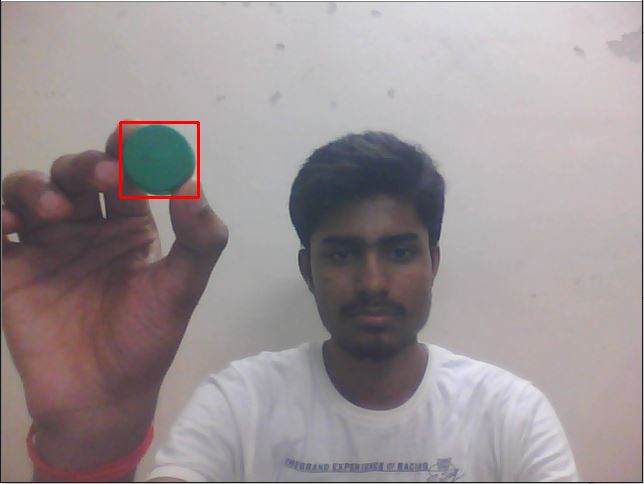
\includegraphics[scale=0.8]{image1.jpg}
	\newline
	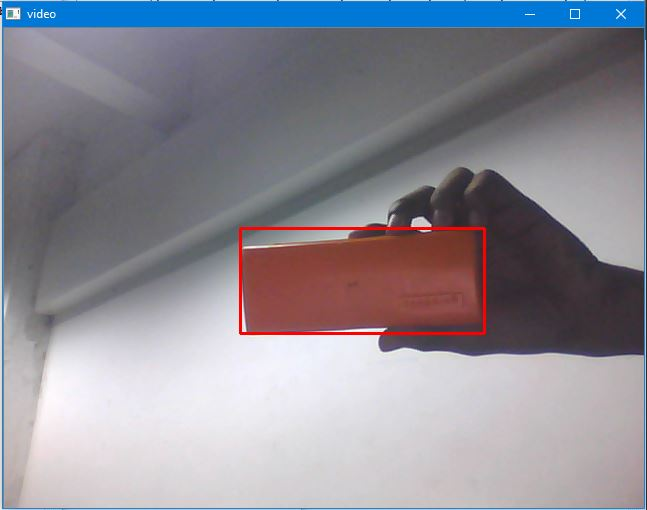
\includegraphics[scale=0.8]{image2.jpg}
	
	\section{References}
		\begin{enumerate}
			\item \url{https://opencv-python-tutroals.readthedocs.io/en/latest/py_tutorials/py_gui/py_drawing_functions/py_drawing_functions.html#drawing-functions}
			\item \url{https://opencv-python-tutroals.readthedocs.io/en/latest/py_tutorials/py_imgproc/py_colorspaces/py_colorspaces.html#converting-colorspaces}
			\item \url{https://opencv-python-tutroals.readthedocs.io/en/latest/py_tutorials/py_imgproc/py_filtering/py_filtering.html#filtering}
			\item \url{https://opencv-python-tutroals.readthedocs.io/en/latest/py_tutorials/py_imgproc/py_contours/py_contours_begin/py_contours_begin.html#contours-getting-started}
			\item \url{https://opencv-python-tutroals.readthedocs.io/en/latest/py_tutorials/py_imgproc/py_contours/py_contour_features/py_contour_features.html#contour-features}
		\end{enumerate}
			
\end{document}



